\section{Experiment 1: theoretical simulation}
As we've seen before, the loudspeaker array in the laboratory can be modelled as an octagon of monopoles (\autoref{WFSdistribution}). If a monopole source is placed outside the area, the loudspeaker array should be able to replicate the field with opposite sign and hence, cancel it inside the octagon. As explained in \autoref{optimization}, the election of points matters when applying the global scalation of loudspeaker coefficients (\autoref{OptScalation}). Therefore, a more or less even distribution of points should be chosen.

As an example, \autoref{figTheoCanc} shows the result for a noise source at position $[-1, 2.5, 0]$, and the optimization applied for the points represented by microphone icons.

\begin{figure}
	\centering
	\reflectbox{\rotatebox[origin=c]{180}{
			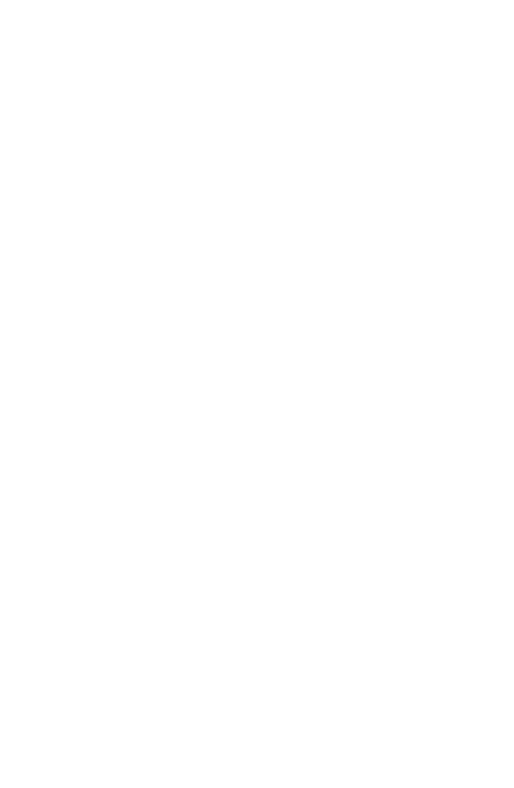
\includegraphics[height=0.3\textheight]{./Img/Experiment1_Example.pdf}
	}}	
	\caption[WFS cancellation]{WFS cancellation. $\rns = [-1, 2.5, 0]$.}
	\label{figTheoCanc}
\end{figure}

To get a sense of what levels of cancellations we can achieve, we test it for different positions of the noise source (\autoref{figNoiseSourcePosTheo}), and the results are shown in \autoref{figCancelDiffNSpostheo}. We've used \autoref{globalCancEq} to calculate the cancellation. As we can see, the closer the noise source is to the centre of the silent area, the better the cancellation. The further it is located, the worse levels of cancellation achieved, but it seems it converges when $R\rightarrow\infty$ to cancellations over $11$ dB. As this is the ideal case, it's reasonable to don't expect better performance in real cases.

\begin{figure}[h]
	\centering
%	\raisebox{0.1\height}{
	\begin{minipage}[b]{0.49\textwidth}
			\centering
			\def\svgwidth{\columnwidth}
			\graphicspath{{Img/}}
			\input{Img/Experiment1_differentNSpositions.pdf_tex}
			\caption[Positions of noise source]{Positions of noise source}
			\label{figNoiseSourcePosTheo}
	\end{minipage}
	\begin{minipage}[b]{0.49\textwidth}
			\centering
		\includegraphics[width=\textwidth]{Img/Experiment1_globalCancDifNSpos_definitive.pdf}
		\caption[Global cancellation. Theoretical model.]{Global cancellation for different positions of the noise source.}
		\label{figCancelDiffNSpostheo}
	\end{minipage}
\end{figure}

Respect to the global correction factor $\Psi$ (\autoref{OptScalation}), in \autoref{figGobalScalationScatter} we can see that, although it changes with distance $R$ and angle $\alpha$, the variation is very small. The mean absolute value is around $0.21$ and the mean phase is approximately $-137^\circ$. 

\begin{figure}
	\centering
	\includegraphics[height=0.3\textheight]{./Img/Experiment1_globalCancScaleFactor.eps}
	\caption[Global correction factor]{Global correction factor}
	\label{figGobalScalationScatter}
\end{figure}

One question that may arise is how much the election of microphones location can change the value of the optimal global scale factor $\Psi$, and so, the cancellation. In order to evaluate that change, we define a new magnitude. Let $\Psi_{\mathit{opt}, i}$ be the optimal global cancellation factor for a given microphone distribution $\pos[matMicro]{,i}$ (\autoref{corrFacti}). Let's define $\cmicro[(i,j)]$ (\autoref{cmicroDifferentPsi}) as the signals received by a set of microphones located at $\pos[matMicro]{,i}$ and correction factor $\Psi_{\mathit{opt}, j}$ (calculated with a different set of microphone locations $\pos[matMicro]{,j}$). Finally, for a given set of microphone locations $\pos[matMicro]{,i}$, let's define the relative global cancellation $C_{\mathit{grel}(i,j)}$ (\autoref{relGlobCanc}) as the relation between the global cancellation achieved with the optimal correction factor for other microphone positions $\Psi_{\mathit{opt}, j}$, and the optimal correction factor for the actual microphone positions $\Psi_{\mathit{opt}, i}$.

\begin{gather}
\Psi_{\mathit{opt}, i} = \argmin_{\Psi} \norm{\Awfs(\pos[matMicro]{,i})\cwfs \Psi + \vec{a}_{\mathit{NS}}(\pos[matMicro]{,i}) \cnsScalar} \label{corrFacti} \\
\cmicro[(i,j)] = \Awfs(\pos[matMicro]{,i})\cwfs \Psi_{\mathit{opt}, j} + \vec{a}_{\mathit{NS}}(\pos[matMicro]{,i}) \cnsScalar \label{cmicroDifferentPsi} \\
C_{\mathit{grel}(i,j)} = \frac{\norm{\cmicro[(i,j)]}^2}{\norm{\cmicro[(i,i)]}^2} \label{relGlobCanc}
\end{gather}

Three sets of microphone locations have been chosen \autoref{figGrids}. The first one is just a microphone in the centre of the octagon. The second one is a ($2.1$x$3.8$)$\si{m}$ rectangular grid with $20$ rows and $20$ columns. The third one is a rectangular grid with the same size as the previous one, but with $100$ rows and $100$ columns. The global correction factor has been calculated with all three of them, and then the cancellation has been calculated with the last grid.  

\section{Experiment 2: GTAC acoustic paths}
The first experiment is a completely theoretical one, although it uses results from previous measures. The acoustic responses in the GTAC laboratory for different points was measured with high precision previously, and the results are published in the website. In total, the measures were done in 360 points distributed in a rectangular grid of size $24$x$15$ and separation of $20 \si{cm}$ between adjacent nodes (\autoref{GTAC360micro}).

\begin{figure}
	\centering
	\reflectbox{\rotatebox[origin=c]{180}{
			\includegraphics[height=0.3\textheight]{./Img/WFSGTAC360microphones.pdf}
	}}	
	\caption[Schematic of measures in GTAC anechoic chamber]{Schematic of measures in GTAC anechoic chamber}
	\label{GTAC360micro}
\end{figure}

%We could apply the optimization already described in \autoref{optimization}, but there is a problem. GTAC responses are measured for loudspeakers in the WFS array, but of course, not for loudspeakers outside the array in arbitrary positions. Hence, we can only guess the acoustic paths by applying the theoretical model (\autoref{acPathTheoric}), in which case we assume that the noise source is isotropic. Then, we apply the optimization process and see how far we can go in the cancellation. Only the first type of optimization is interesting since the position of the noise loudspeaker is known.

GTAC responses are measured for loudspeakers in the WFS array, but of course, not for loudspeakers outside the array in arbitrary positions. Hence, we can only guess the acoustic paths by applying the theoretical model (\autoref{acPathTheoric}), in which case we assume that the noise source is isotropic.

Results are shown in \reffig{}. Different positions have been used. As we can see, cancellations of X dB are easy to achieve.



\section{Experiment 3: lab recording}
